\documentclass[11pt,a4paper]{article}
\usepackage[margin=2.3cm]{geometry}
\usepackage{amsmath,amssymb}
\usepackage{graphicx}
\usepackage{booktabs}
\usepackage{array}
\usepackage{float}
\setlength{\intextsep}{8pt plus 2pt minus 2pt}
\usepackage[font=small,labelfont=bf]{caption}
\usepackage[colorlinks=true,allcolors=blue!50!black]{hyperref}
\usepackage{xcolor}
\newcommand{\todo}[1]{\textcolor{red!70!black}{[TO DO: #1]}}
\newcommand{\refpending}[1]{\textcolor{red!70!black}{[reference pending: #1]}}

\title{Solver configuration in VOF simulations of Taylor bubbles on film-resolving stretched meshes}
\author{Sebbi Adam Kasambula\\[3pt]
{\normalsize Link\"oping University, SE-581 83 Link\"oping, Sweden}\\[1pt]
{\normalsize \href{mailto:sebbi.a.kasambula@gmail.com}{sebbi.a.kasambula@gmail.com}}}
\date{November 2026}

\begin{document}
\maketitle

\begin{abstract}
Taylor bubbles at Eo = 300, 100 and 20 and Nf = 1000, 50 and 500 were simulated with the volume of fluid method in OpenFOAM and Ansys Fluent on identical axisymmetric meshes stretched to resolve the film. Fr in Fluent differed from OpenFOAM by +2.5\%, +20.8\% and $-10.7\%$, all inside the scatter of the correlation of Viana et al. A mesh of square cells moved Fr at Eo = 300 by 3.6\% in OpenFOAM and 0.4\% in Fluent. At Eo = 100 the differing settings were changed one at a time and compared with the sharp-interface simulations of Abubakar and Matar and the nearest measurement, which the OpenFOAM baseline underestimated by 13.7\% and 18.2\%. Solving the momentum equation before the pressure correction in OpenFOAM raised Fr by 5.2\%, close to the 4.1\% from halving the time step. Geometric advection with isoAdvector then brought Fr and the film to within 1.0\% and 0.4\% of the sharp-interface values. Changing the surface tension term of OpenFOAM to the density-weighted form that Fluent uses lowered Fr by 29.5\%. At Eo = 100, Fr in every run lay within 3.3\% of the value that laminar film theory gives for its film. The grid uncertainty of Fr, 5\% to 33\%, was comparable to the differences from the references, while the baseline film lay 4.5\% below the sharp-interface film against an uncertainty of 2.5\%. The same settings lowered Fr at Eo = 300 by 3.8\% and left it within the fit error at Eo = 20.
\end{abstract}

\noindent\textit{Keywords}\quad Taylor bubble, volume of fluid, OpenFOAM, Ansys Fluent, solver settings, falling film, verification and validation

\section{Introduction}

A Taylor bubble is a long gas bubble that nearly fills a vertical pipe and rises through the liquid, with a thin liquid film between the gas and the wall. Resolving this film in a volume of fluid (VOF) simulation \cite{hirt1981volume} requires cells much thinner at the wall than at the axis, so the mesh is stretched in the radial direction and the cells at the interface have large aspect ratios. Surface tension in standard VOF also produces spurious currents, which are velocities at the interface with no physical origin \cite{harvie2006analysis,popinet2018numerical}. This paper asks how much of the difference between two VOF codes in the rise velocity and film thickness of a Taylor bubble can be traced to their solver settings.

The question matters because a grid study refines one family of meshes in one code, so it may be unable to see an error set by the cell shape or by the code. Harvie et al.\ \cite{harvie2006analysis} found that parasitic currents do not decrease with mesh refinement or with a smaller time step. Abadie et al.\ \cite{abadie2015combined} reported a slip velocity error for Taylor flow in a microchannel at Ca $\approx$ 0.005 that moved from 20.44\% to 18.71\% between two meshes stretched towards the wall with their VOF method, against 1.88\% to 0.31\% with their level set method. Ara\'ujo et al.\ \cite{araujo2012wide} used uniform meshes with an aspect ratio of about one and describe this as advisable for the geometric reconstruction.

Two codes have also been compared on the same problem. Silva et al.\ \cite{silva2020numerical} ran a Taylor bubble through a microchannel in OpenFOAM and in Fluent, with an imposed flow and no gravity, on an axisymmetric Fluent mesh and a $5^\circ$ OpenFOAM wedge. At Ca = 0.03 the two OpenFOAM solvers gave a film 2.2 to 2.3 times the correlation value while Fluent matched it. Marschall et al.\ \cite{marschall2014validation} compared four interface capturing and tracking codes with an X-ray measurement of a Taylor bubble in a square channel, and took the bubble length and the minimum film thickness as the quantities to compare. Neither Fluent nor \texttt{interFoam} took part. Hysing et al.\ \cite{hysing2009quantitative} set a two-dimensional rising bubble benchmark, and CFX, Comsol, Fluent and three research codes disagreed on the same problem.

The settings that differ between the two codes have each been studied on their own. Horgue et al.\ \cite{horgue2012suitable} ranked the Fluent volume fraction schemes by the number of cells the interface spans, and found that Geo-Reconstruct holds it between 1.86 and 2.05 cells at any Courant number while the least compressive of the schemes spread it over 3 to 14 cells. Cifani et al.\ \cite{cifani2016comparison} compared the interface compression of \texttt{interFoam} with a PLIC reconstruction and report that the compression does not converge under refinement while the reconstruction does. Gamet et al.\ \cite{gamet2020validation} measured the curvature error and the spurious currents of \texttt{interFoam} against the isoAdvector solvers, and found that the gradient curvature error of \texttt{interFoam} grows under refinement while the reconstructed distance function is about two orders better, with the currents of plicRDF about two orders below those of MULES. Each of these measures a scheme change inside one code. None of them measures how much of a difference between two codes such a change accounts for.

The study covers one static bubble, run in OpenFOAM, and three rising bubbles, run in OpenFOAM and in Ansys Fluent on matching meshes. Two of the rising cases carry a grid study, the second of them in both codes, so the difference between the codes is reported in units of the grid uncertainty of the case it is measured at. A test of mesh shape under the same conditions in both codes is followed by a comparison of the two codes at all three rising cases. At the case where the codes differ most, each setting that differs between them was then changed on its own, one code at a time, against decision rules fixed before those runs were started. At that case the rise velocity and the film are also compared with an independent sharp-interface method and a measurement, with the uncertainty of each comparison, and the film with laminar film theory. The OpenFOAM configuration closest to these references was then run at the other two cases.

\section{Cases and reference values}

The flow is set by the E\"otv\"os number and the inverse viscosity number,
\begin{equation}
\mathrm{Eo} = \frac{\Delta\rho\, g D^2}{\sigma}, \qquad
\mathrm{Nf} = \frac{\sqrt{D^3 g\, \Delta\rho\, \rho_l}}{\mu_l},
\end{equation}
and the rise velocity $U_b$ is reported as $\mathrm{Fr} = U_b/\sqrt{gD}$. The Morton number $\mathrm{Mo} = \mathrm{Eo}^3/\mathrm{Nf}^4$ depends on the fluids alone, and the bubble Reynolds number is $\mathrm{Re} = \mathrm{Fr}\,\mathrm{Nf}$. All runs use $D = 1$ m, $\rho_l = 1$ kg/m$^3$ and $g = 1$ m/s$^2$, so a speed of 1 m/s equals $\sqrt{gD}$. The density ratio is 1000 and the viscosity ratio is 100. Table~\ref{tab:cases} lists the cases. Case S is a static bubble of radius 0.25 $D$ without gravity, with the surface tension and viscosities of Eo = 10 and Nf = 2000, run for ten capillary times.

\begin{table}[H]
\centering
\caption{Cases and reference values. Re uses the Fr of Viana et al. The film correlation applies above Eo = 40.}
\label{tab:cases}
\begin{tabular}{lrrrrccc}
\toprule
Case & Eo & Nf & Mo & Re & Fr (Viana) & $\delta/D$ (Llewellin) & $Z/D$ \\
\midrule
S & 10 & 2000 & $6.3\times10^{-11}$ & & static & & \\
T1 & 300 & 1000 & $2.7\times10^{-5}$ & 338 & 0.3384 & 0.0615 & 2.0 \\
T2 & 100 & 50 & 0.16 & 12.5 & 0.2504 & 0.1394 & 0.2 \\
T3 & 20 & 500 & $1.3\times10^{-7}$ & 139 & 0.2770 & & 1.0 \\
\bottomrule
\end{tabular}
\end{table}

The reference rise velocity is equation (23) of Viana et al.\ \cite{viana2003universal}, which they state predicts Fr with an error of $\pm 0.05$ at most. That is 15\% of Fr at T1 and 20\% at T2, so each result is judged against this scatter. The reference film thickness is equation (4.2) of Llewellin et al.\ \cite{llewellin2012thickness}. The length $Z$ is their development length, equation (2.27). Film thickness is averaged from the larger of 1.5 $D$ and $Z$ below the nose to 0.5 $D$ above the tail. In OpenFOAM the film is measured from the flat wall face of the wedge, which lies 0.4995 $D$ from the axis in its mid-plane.

At T2 a second reference comes from the steady simulations of Abubakar and Matar \cite{abubakar2021taylor}, who solved the axisymmetric equations with a sharp interface by the finite element method and took the gas as a region of constant pressure with no density or viscosity. Their Figure 6a gives Fr at Eo = 100 for Nf = 40, 60 and 80. The values read from the figure are 0.2336, 0.2692 and 0.2879, and the correlation of Viana et al.\ plotted in the same figure, read in the same way, came within 0.0005 of its equation. Interpolation to Nf = 50 gives 0.2531, and three interpolation rules give 0.2514 to 0.2544. Their Figure 7b gives the film thickness of the same runs, 0.1458, 0.1351 and 0.1266 $D$, and the lines of their film relation in that figure, read in the same way, came within 0.0002 of the relation. Interpolation gives a film of 0.1403 $D$ at Nf = 50, with 0.1401 to 0.1405 from the three rules. Against the measured Fr of 0.303 at Eo = 98.3 and Nf = 89 \cite{bugg2002velocity} their method gave 3.4\% less, and that experiment did not measure the film. So this reference is itself a simulation.

The supplementary appendix of Viana et al.\ \cite{viana2003universal} lists one measurement close to T2, by White and Beardmore in a 95\% glycerol solution at Nf = 50.3 and Eo = 128.4, with Fr = 0.2671. At this Nf the correlation of Viana et al.\ changes Fr by 0.9\% between Eo = 100 and 128.4. The three other measurements within about 40\% of T2 in both Nf and Eo lie 11.8\% below to 7.0\% above the correlation. No measurement in the appendix lies within 25\% of T1 or T3 in both Nf and Eo.

\section{Method}
\label{sec:method}

The flow was modelled as laminar and axisymmetric, in a pipe of length 20 $D$ with a closed bottom, an open top and no-slip walls. The liquid starts at rest. The bubble starts as a capsule near the bottom of the pipe, with a radius close to the pipe radius minus the expected film. OpenFOAM v2412 \cite{weller1998tensorial} (\texttt{interFoam}) used a one-cell wedge of $5^\circ$, because it has no axisymmetric mode. Fluent 2024 R1 used its axisymmetric formulation. The meshes of the rising cases are the same in both codes, and their node positions agree within $10^{-8}$ $D$.

Both codes solve one set of equations for the two fluids, with the liquid volume fraction $\alpha$ marking each cell,
\begin{align}
\frac{\partial \alpha}{\partial t} + \nabla\cdot(\alpha\mathbf{u}) &= 0, \label{eq:alpha}\\
\nabla\cdot\mathbf{u} &= 0, \\
\frac{\partial (\rho\mathbf{u})}{\partial t} + \nabla\cdot(\rho\mathbf{u}\mathbf{u}) &= -\nabla p + \nabla\cdot\left[\mu\left(\nabla\mathbf{u}+\nabla\mathbf{u}^{T}\right)\right] + \rho\mathbf{g} + \sigma\kappa\nabla\alpha, \label{eq:mom}
\end{align}
where $\rho = \alpha\rho_l + (1-\alpha)\rho_g$, $\mu = \alpha\mu_l + (1-\alpha)\mu_g$ and the curvature is $\kappa = -\nabla\cdot(\nabla\alpha/|\nabla\alpha|)$. The last term in equation~\eqref{eq:mom} is the continuum surface force model of Brackbill et al.\ \cite{brackbill1992continuum}, in the form OpenFOAM uses. Fluent multiplies this term by $2\rho/(\rho_l+\rho_g)$ \cite{ansys2024fluenttheory}, the density-weighted form given in the same paper, so the weight runs from about 0.002 in the gas to about 2 in the liquid. In OpenFOAM equation~\eqref{eq:alpha} carries an added term $\nabla\cdot[\mathbf{u}_r\alpha(1-\alpha)]$ that compresses the interface, with $\mathbf{u}_r$ scaled by $c_\alpha$. Fluent reconstructs a sharp, piecewise-linear interface in each cell from $\alpha$ and its gradient before it computes the flux \cite{ansys2024fluenttheory}.

The two codes differ in how they treat the interface, and Table~\ref{tab:solver} lists the settings of each. Both codes correct the pressure with the PISO algorithm of Issa \cite{issa1986solution}. Fluent solves the momentum equations before the pressure correction in each of its iterations \cite{ansys2024fluenttheory}, which is the step that the momentum predictor switches on in OpenFOAM. In OpenFOAM the time step was adjusted during each run, with a maximum Courant number of 0.5 and a maximum interface Courant number of 0.2, under the capillary limit of Brackbill et al.\ \cite{brackbill1992continuum}. The capillary limit was halved for case S. In Fluent the time step grew from $10^{-4}$ s over the first 40 or so steps to a cap equal to the OpenFOAM capillary limit to within about 1\% on the stretched meshes, and then stayed at the cap. On the square mesh it was set by a Courant number of 0.5.

\begin{table}[H]
\centering
\small
\caption{Numerical settings.}
\label{tab:solver}
\setlength{\tabcolsep}{3pt}
\begin{tabular}{>{\raggedright\arraybackslash}p{0.25\linewidth}>{\raggedright\arraybackslash}p{0.33\linewidth}>{\raggedright\arraybackslash}p{0.33\linewidth}}
\toprule
 & OpenFOAM & Fluent \\
\midrule
Version & v2412, \texttt{interFoam} & 2024 R1 \\
Geometry & $5^\circ$ wedge, one cell thick & Axisymmetric formulation \\
Volume fraction & MULES, $c_\alpha = 1$, van Leer & Geo-Reconstruct \\
Momentum & Linear upwind & Second-order upwind \\
Pressure interpolation & & PRESTO! \\
Coupling & One outer loop, 3 pressure correctors, no momentum predictor & PISO, momentum and pressure in each of 20 iterations per step \\
Time stepping & Euler, adaptive step & Adaptive, held at the cap \\
Surface tension & $\sigma\kappa\nabla\alpha$ & $\sigma\kappa\nabla\alpha \cdot 2\rho/(\rho_l+\rho_g)$ \\
Wall adhesion, curvature smoothing & Off & Off \\
\bottomrule
\end{tabular}
\end{table}

Fluent used all 20 iterations in every time step at T1, and the continuity residual ended each step at about $4\times10^{-3}$. To test this, the run was continued from 20 s for 2 s with 40 iterations per step, which brought the residual to about $1\times10^{-5}$. Over these 2 s Fr was 0.3379, against 0.3376 over 5 to 20 s, a difference of 0.08\% against a standard error of 0.30\% for the shorter fit. The film changed by 0.4\%. The Fluent runs kept 20 iterations per step.

Table~\ref{tab:mesh} lists the meshes. The stretched meshes have uniform axial spacing and a radial grading of 0.25 towards the wall, which gives a maximum aspect ratio of about 17. The baseline of 96 radial by 480 axial cells places 22 cells within 0.0615 $D$ of the wall, the T1 film from Llewellin et al.

\begin{table}[H]
\centering
\small
\caption{Meshes. $\Delta x/\Delta r$ is the largest cell aspect ratio, at the wall. In film counts the cells within 0.0615 $D$ of the wall.}
\label{tab:mesh}
\setlength{\tabcolsep}{3pt}
\begin{tabular}{lrrrrr}
\toprule
Mesh & Radial & Axial & Cells & $\Delta x/\Delta r$ & In film \\
\midrule
Coarse & 69 & 343 & 23 667 & 17.5 & 16 \\
Medium & 96 & 480 & 46 080 & 17.3 & 22 \\
Fine & 134 & 672 & 90 048 & 17.3 & 30 \\
Square & 48 & 1920 & 92 160 & 1.0 & 6 \\
S stretched & 96 & 96 & 9 216 & 17.3 & \\
S uniform coarse & 12 & 96 & 1 152 & 1.0 & \\
S uniform fine & 48 & 384 & 18 432 & 1.0 & \\
\bottomrule
\end{tabular}
\end{table}

Table~\ref{tab:runs} lists the rising runs on the medium mesh. The continuity residual is the residual Fluent reports for the mass equation at the end of each time step, after its iterations, and the table gives its median over the steps. The table also gives the viscous diffusion number $\nu\Delta t/\Delta r^2$ of the wall cell, 0.0024 $D$ high, for the liquid and for the gas at the time step cap.

\begin{table}[H]
\centering
\caption{Rising runs on the medium mesh. Gas drift is the largest change of the gas volume during a run.}
\label{tab:runs}
\small
\setlength{\tabcolsep}{3pt}
\begin{tabular}{lcccccccc}
\toprule
 & \multicolumn{2}{c}{End time (s)} & Time step & Fluent continuity & \multicolumn{2}{c}{Gas drift (\%)} & \multicolumn{2}{c}{$\nu\Delta t/\Delta r^2$, wall} \\
Case & OpenFOAM & Fluent & (s) & residual & OpenFOAM & Fluent & Liquid & Gas \\
\midrule
T1 & 39.4 & 20.0 & $9.1\times10^{-4}$ & $4\times10^{-3}$ & 0.0029 & $1\times10^{-5}$ & 0.16 & 1.6 \\
T2 & 53.2 & 21.0 & $8.5\times10^{-4}$ & $3\times10^{-4}$ & 0.0071 & $9\times10^{-5}$ & 2.95 & 29.5 \\
T3 & 48.1 & 23.2 & $2.6\times10^{-4}$ & $7\times10^{-6}$ & 0.0385 & $3\times10^{-6}$ & 0.089 & 0.89 \\
\bottomrule
\end{tabular}
\end{table}

The initial gas volume cannot match exactly, since OpenFOAM fills whole cells and the outermost row of gas cells holds 1.4\% to 2.4\% of the gas. With the OpenFOAM gas fraction scaled to the volume of the full pipe, the differences are $-0.59\%$ at T1, $+0.82\%$ at T2 and $+0.46\%$ at T3. On the square mesh at T1 the difference was $+1.04\%$.

Each snapshot was measured in the same way in both codes. The nose is the highest point on the axis where $\alpha$ crosses 0.5, interpolated between cell centres. The bubble is the region of cells with $\alpha < 0.5$ connected through cell faces to the nose, and its length runs from the nose to the lowest cell of this region on the axis, called the tail. Gas outside the bubble is the gas below the tail that does not belong to this region, given as a share of all the gas. The part of it within 2 $D$ below the tail is also given on its own. Smeared gas is the gas held in cells with a gas fraction below 0.5. The largest speeds are taken over all cells and over the liquid cells with $\alpha > 0.99$. The film window of Section~2 starts 0.5 $D$ above the first liquid cell met going down the axis from the nose. Over a time window, films, lengths and gas shares are means over the snapshots and speeds are medians. The field figures show the speed mirrored about the axis, with the interface at a gas fraction of 0.5 in white and the nose at $x = 0$ unless stated.

\section{Verification}

\subsection{Static bubble}

Case S tested the surface tension implementation. In OpenFOAM the pressure jump averaged 0.728 Pa against 0.799 Pa from the Laplace law, an error of $-8.8\%$, with a standard deviation of 0.044 Pa. Up to $t = 1$ s the jump stayed 6.7\% to 8.3\% below the Laplace value on all three meshes of case S (Section~\ref{sec:shape}), also on the uniform mesh whose axial cell is four times smaller, so refining the mesh did not remove the error. Deshpande et al.\ \cite{deshpande2012evaluating} also conclude that the pressure jump does not converge to the exact value. The peak liquid velocity was 0.38 to 0.79 m/s, with no decay over the run. The gas volume drifted by $+0.01\%$ over 4 s.

\subsection{Mass conservation and time step}
\label{sec:dt}

Gas volume drifted by no more than 0.0082\% in any OpenFOAM T1 run and by $1\times10^{-5}\%$ in Fluent.

The time step at T1 was limited by the capillary constraint of Brackbill et al.\ \cite{brackbill1992continuum}. This gave a maximum step of $9.12\times10^{-4}$ s on the medium mesh. The interface Courant limit of 0.2 would have allowed a step about 1.4 times larger and set the step at times, so the capillary limit itself was halved to test the margin. With the halved limit Fr changed from 0.3300 to 0.3306. The difference of 0.18\% is below the fine-grid GCI of 1.06\%. At T2 the same test raised Fr over 5 to 8.4 s by 4.1\% (Section~\ref{sec:configs}). The validation runs kept the full capillary limit.

\subsection{Grid convergence}
\label{sec:grid}

The three stretched meshes of Table~\ref{tab:mesh}, with a refinement ratio of about 1.4, were run at T1 in OpenFOAM and at T2 in both codes, and the GCI \cite{Celik2008} was computed for Fr. At T1, with Fr fitted to the nose from 5 s to the end of the run, the fine-grid GCI was 1.06\% and the GCI of the medium mesh, which is used for the comparisons, about 2.3\%. The film changed by 0.3\% from the medium to the fine mesh. At T2, with Fr fitted from 5 to 8.4 s and the time step scaled with the cell size, the GCI of the medium mesh was 5.0\% in Fluent and 20.5\% in OpenFOAM, where the observed order of 0.62 lies below the range of 1.0 to 2.5. For the film the GCI of the medium mesh was 2.5\% in OpenFOAM, with an order of 1.7. In Fluent the change of the film grew from 0.45\% between the coarse and medium meshes to 0.80\% between the medium and fine meshes, so the three meshes give no order for it. OpenFOAM with geometric advection and the momentum predictor (Section~\ref{sec:configs}) was also run at T2 on the coarse and fine meshes. On the coarse mesh Fr was 1.5\% above the medium mesh. On the fine mesh the bubble stretched from the start, and between 5.0 and 5.2 s its front separated as a second bubble holding 14\% of the gas, so no Fr is given for it. The momentum predictor alone was also run on the coarse and fine meshes. On the coarse mesh Fr was 4.4\% above the medium mesh, against 4.1\% without the predictor. On the fine mesh the bubble stretched from the start, and its front separated twice, between 2.6 and 2.8 s with 18\% of the gas and between 3.6 and 3.8 s with 15\%, so no Fr is given for it either. In both runs on the fine mesh with the momentum predictor, the largest gas speed inside the bubble, next to the axis, reached 25 and 122 m/s before the bubble separated, against at most 1.1 m/s in every other run at T2, including the fine mesh without the predictor. In both runs the same sequence occurred. Up to about 0.06 s they followed the other runs at T2. The largest initial residual of the pressure equation then grew about tenfold every 0.03 s, from about 0.002 to about 0.1 and 0.2 by 0.13 s, while it stayed near 0.001 in every other run at T2. From about 0.14 s a smooth flow of gas along the axis appeared inside the bubble and changed direction between snapshots, and by 2 s more than half of the gas cells of the bubble moved faster than 2 m/s. The bubble then stretched and its front separated. At 2.6 s the gas of the bubble without the predictor spanned 2.0 to 5.3 $D$ above the bottom of the pipe, while the gas of the bubble with it spanned 2.0 to 8.1 $D$, with a neck near 6.2 $D$ where the gas was fastest. At 2.8 s its front, holding 18\% of the gas, had separated and lay between 6.8 and 8.7 $D$ (Figure~\ref{fig:split}). This happened only with the momentum predictor on and only on the fine mesh, with the time step held at the capillary limit. Deshpande et al.\ \cite{deshpande2012evaluating} found that spurious currents in \texttt{interFoam} can grow until the flow becomes unstable without any Courant limit being exceeded, that refining the grid raises the spurious velocity scale, and that the low density of the light phase amplifies an imbalance that comes from the residuals of the pressure equation. With the cell sizes of these meshes the spurious velocity scale of the gas, $\sqrt{\sigma/(\rho_g\Delta x)}$, is about 30 to 60 m/s, the order of the gas speeds reached here. Gupta et al.\ \cite{gupta2009cfd} found that their finest grids increased the non-physical pressure jumps across the interface, and Andredaki et al.\ \cite{andredaki2021accelerating} describe a jet of gas that formed inside accelerating Taylor bubbles and travelled to their front. Why only the fine mesh with the momentum predictor became unstable was not established.

\begin{figure}[H]
\centering
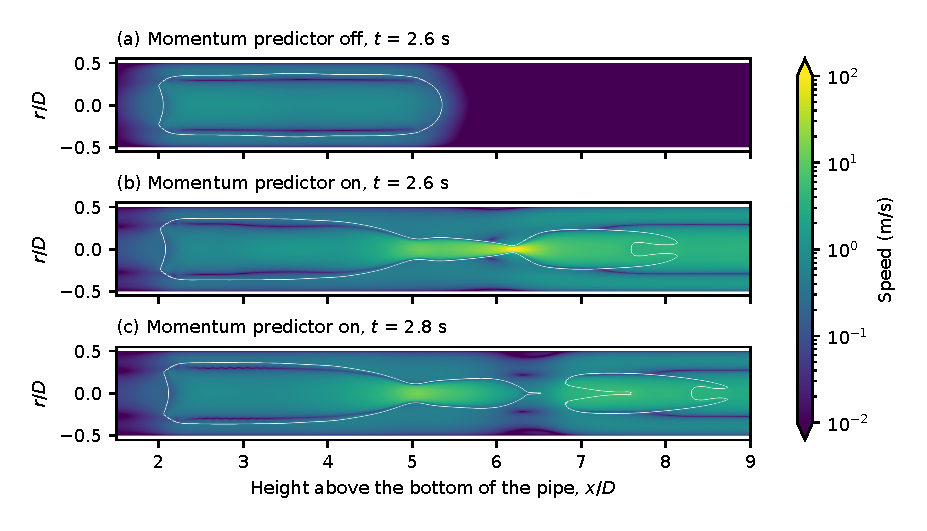
\includegraphics[width=0.75\linewidth]{figures/fig_t2_split.eps}
\caption{Speed at T2 on the fine mesh on a log scale, (a) without the momentum predictor at 2.6 s, (b) with it at 2.6 s and (c) with it at 2.8 s. The bubble rises to the right.}
\label{fig:split}
\end{figure}

\section{Effect of mesh shape}
\label{sec:shape}

A uniform mesh of 92 160 square cells was then run under the same conditions, with about 6 cells across the film. It gave Fr = 0.3390. That value lies 3.8\% above the fine stretched mesh, about 3.6 times the fine-grid GCI. The square mesh has no grid study of its own. This is an observation that the grid study alone did not show. The square mesh was still settling from 5 to 10 s (Figure~\ref{fig:frsq}), and from 10 s to the end it gave Fr = 0.3385, which is 3.5\% above the fine mesh over the same window (0.3269). The film over 5 to 20 s was 0.0662 $D$, from 15 of the 24 samples, against 0.0655 $D$ on the fine stretched mesh. Against the stretched meshes, the square mesh changes three things at once. The cells have an aspect ratio of one, the axial cell is 4 times smaller than on the medium mesh, and the film holds about 6 cells against 22, so the shift cannot be assigned to the aspect ratio alone. This one run cannot show which mesh is closer to the true value, since the square mesh has few cells in the film. Figure~\ref{fig:filmmesh} shows the two meshes across the film 2.5 $D$ behind the nose at 19.7 s. There the film was 0.0646 $D$ thick on the stretched mesh and 0.0644 $D$ on the square mesh, which spans 22.8 and 6.2 cells.

Fluent was run on the same square mesh, starting from the same gas volume as its stretched run to within 0.002\%. Over 5 to 20 s Fluent gave Fr = 0.3391, which is 0.4\% above the Fluent stretched mesh over the same window (0.3376), and the film was 0.0654 $D$ against 0.0658 $D$. OpenFOAM moved by 3.6\% between the same two meshes over the same window, from 0.3293 to 0.3411. Fluent was 2.5\% above OpenFOAM on the stretched mesh and 0.6\% below it on the square mesh. Fluent took a time step of about $2.3\times10^{-3}$ on the square mesh, set by the Courant limit, and the continuity residual at the end of each step was higher than on the stretched mesh. Figure~\ref{fig:frsq} shows Fr over 5 s windows on both meshes in both codes, from straight line fits to the nose position, plotted at the window centre.

\begin{figure}[H]
\centering
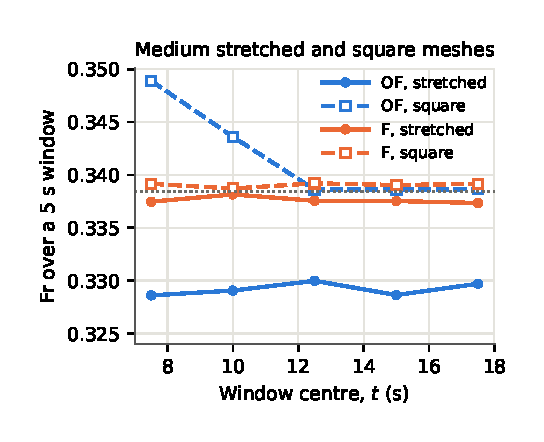
\includegraphics[width=0.55\linewidth]{figures/fig_fr_sq.eps}
\caption{Fr at T1 over 5 s windows on the stretched and square meshes in OpenFOAM (OF) and Fluent (F). Dotted, the value of Viana et al.}
\label{fig:frsq}
\end{figure}

\begin{figure}[H]
\centering
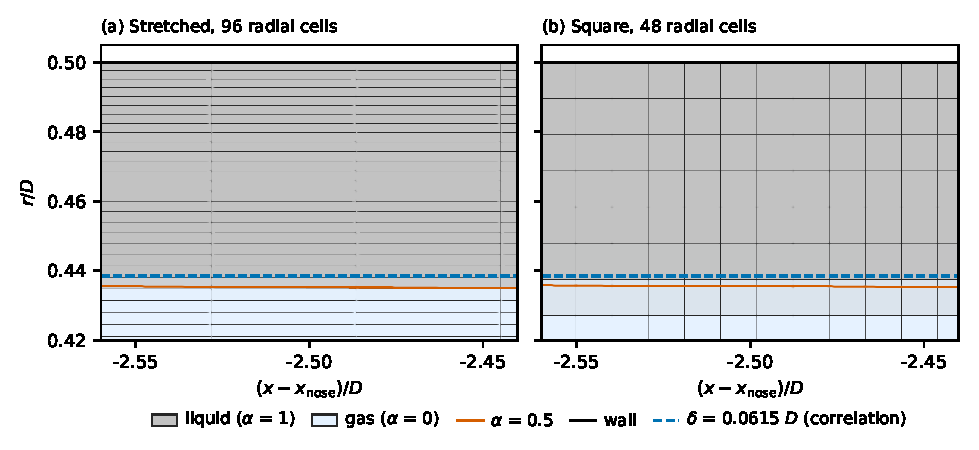
\includegraphics[width=0.75\linewidth]{figures/fig_film_mesh.eps}
\caption{Cells across the T1 film in OpenFOAM on (a) the stretched mesh and (b) the square mesh. Broken line, the film of Llewellin et al.}
\label{fig:filmmesh}
\end{figure}

Static runs on case S were used to look at the currents directly. The stretched mesh was compared with two meshes of aspect ratio about one (Table~\ref{tab:mesh}), each run to $t = 1$ s, using the time mean of the maximum speed over 0.3 to 1 s. The 96 by 12 mesh keeps the axial cell of the stretched mesh, so it has one eighth of the cells and radial cells 8 times larger on average. The mean maximum speed fell by a factor of about 5, and the liquid peak by a factor of 3 to 4. Figure~\ref{fig:sfields} shows the two fields. The 384 by 48 mesh also refines the axial cell by four, and it lowered the mean maximum speed by a factor of about 4. On all three meshes the pressure jump stayed below the 0.799 Pa of the Laplace law. Neither uniform mesh isolates the aspect ratio, since the cell size changes with it. Tightening the pressure tolerance changed the mean maximum speed and the mean pressure jump by 0.3\%, and a tenfold rise in both viscosities lowered the liquid peak by a factor of about 2.1.

\begin{figure}[H]
\centering
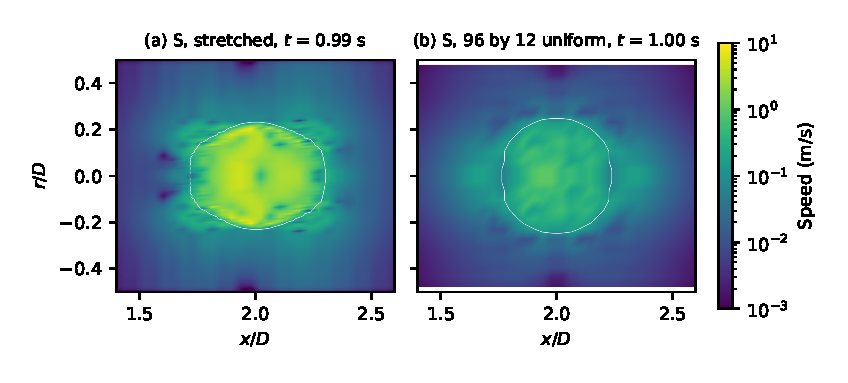
\includegraphics[width=0.75\linewidth]{figures/fig_s_fields.eps}
\caption{Speed of case S on a log scale on (a) the stretched mesh and (b) the uniform mesh with the same axial cell.}
\label{fig:sfields}
\end{figure}

In the rising bubble the largest speeds come from the flow itself. Figure~\ref{fig:t1fields} shows the speed field at T1 on both meshes in both codes near 19.7 s (19.2 s for Fluent on the square mesh), and Figure~\ref{fig:t1mesh} gives the change of each quantity over 5 to 20 s from the stretched to the square mesh, as a percentage of the stretched-mesh value. Its three speeds are the largest speed in all cells, the largest speed in the liquid and the volume-weighted mean speed of the pure gas cells of the bubble. The largest speed lay inside the bubble in 23 of 24 snapshots in OpenFOAM on the stretched mesh, 17 of 24 on the square mesh, and 23 of 28 and 9 of 11 in Fluent. Between the two meshes the medians of the largest speed and of the largest liquid speed changed by at most 1.5\% in both codes. In largest speed the snapshots of the figure lie between the 4th and the 82nd percentile of their runs, so the medians are the values to compare.

\begin{figure}[H]
\centering
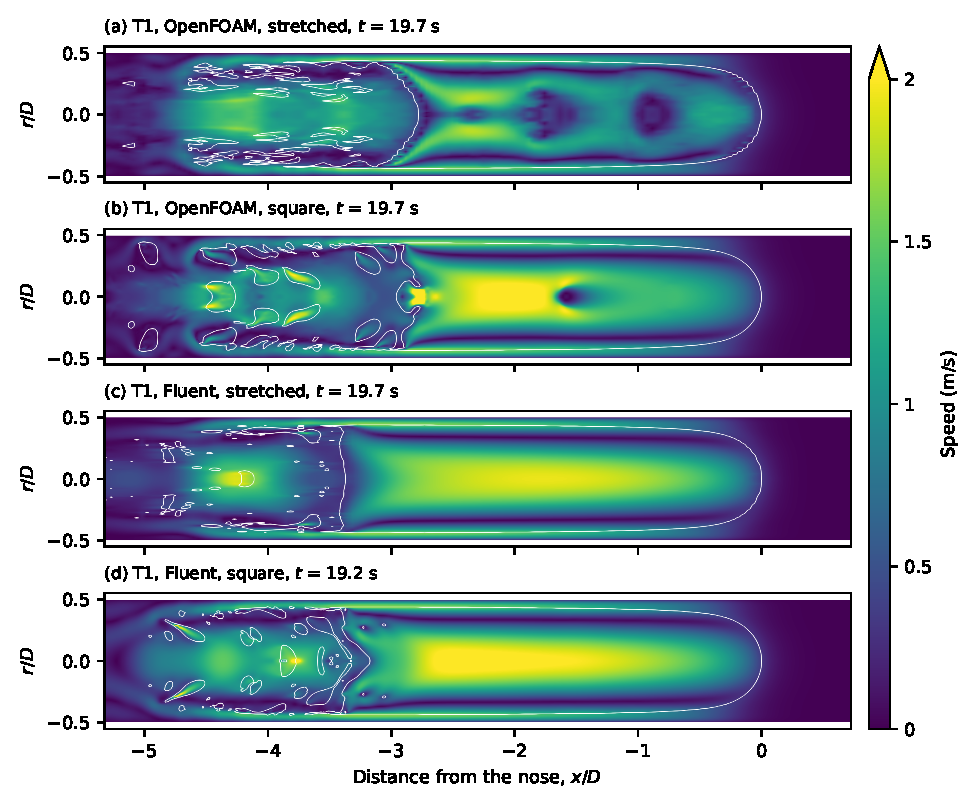
\includegraphics[width=0.75\linewidth]{figures/fig_t1_fields.eps}
\caption{Speed at T1 near 19.7 s on the stretched and square meshes. Speeds above 2 m/s are shown in the top colour.}
\label{fig:t1fields}
\end{figure}

\begin{figure}[H]
\centering
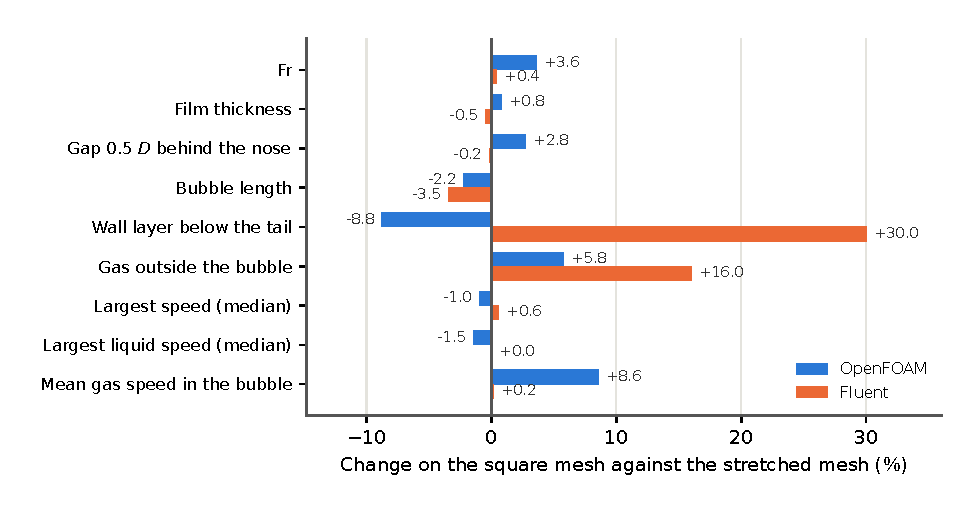
\includegraphics[width=0.75\linewidth]{figures/fig_t1mesh.eps}
\caption{Change at T1 from the stretched to the square mesh over 5 to 20 s.}
\label{fig:t1mesh}
\end{figure}

Gas left the tail in all four runs, and the white lines behind the tail in Figure~\ref{fig:t1fields} mark it. On both meshes OpenFOAM held about twice the share of the gas outside the bubble that Fluent held, and most of it lay within 2 $D$ below the tail. The square mesh raised this share by about 1 percentage point in both codes, which is 6\% of the OpenFOAM share and 16\% of the Fluent share.

Figure~\ref{fig:t1outline} overlays the interface of the same four snapshots, OpenFOAM in the upper half and Fluent in the lower half, with the OpenFOAM radius moved out by 0.0005 $D$ so that both walls lie at 0.5 $D$. The gap between the interface and the wall half a diameter behind the nose changed by 2.8\% between the meshes in OpenFOAM and stayed at 0.110 $D$ in Fluent. The square mesh made the bubble 2.2\% shorter in OpenFOAM and 3.5\% shorter in Fluent, and the Fluent bubble was 10.5\% longer than the OpenFOAM bubble on the stretched mesh and 9.1\% longer on the square mesh. In more than 90\% of the snapshots of each run a thin layer of gas, joined to the bubble, ran down the wall more than 0.1 $D$ below the tail. In the figure this layer is the part of each outline that runs along the wall beyond the tail. On the square mesh it reached 9\% less far below the tail in OpenFOAM and 30\% further in Fluent (Figure~\ref{fig:t1mesh}).

\begin{figure}[H]
\centering
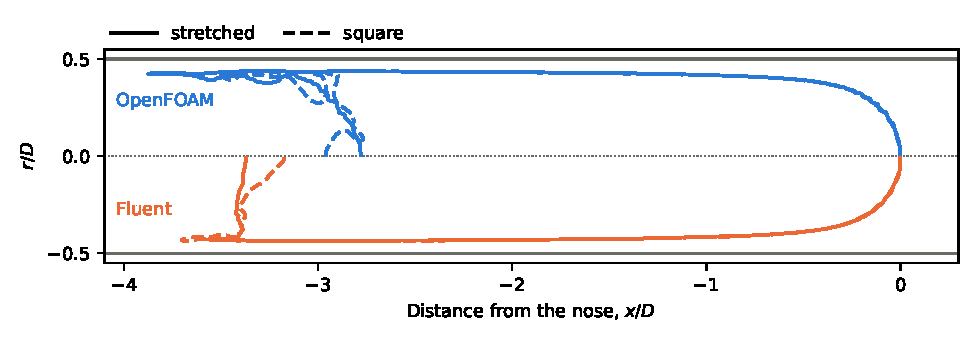
\includegraphics[width=\linewidth]{figures/fig_t1_outline.eps}
\caption{Bubble outline at T1 in the snapshots of Figure~\ref{fig:t1fields}, stretched mesh solid and square mesh broken.}
\label{fig:t1outline}
\end{figure}

\section{Comparison of OpenFOAM and Fluent}

The two codes were compared at T1 to T3 on the medium stretched mesh over 5 to 20 s, with the same fluid properties and time step (Table~\ref{tab:runs}), and Figures~\ref{fig:cases} and~\ref{fig:cases2} show the results.

\begin{figure}[H]
\centering
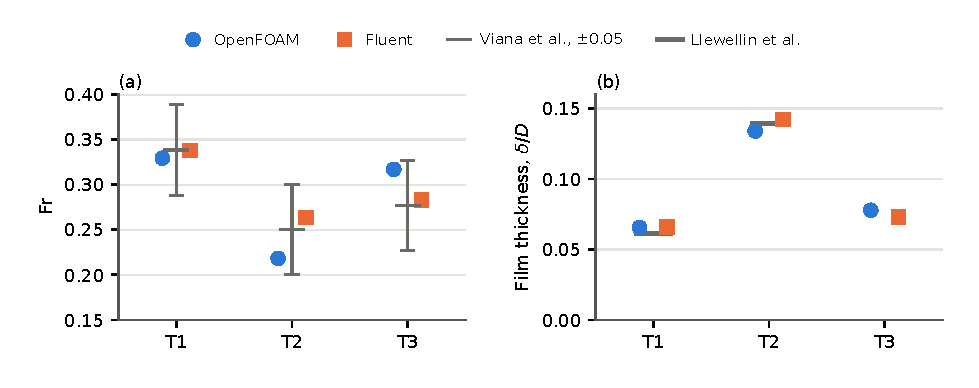
\includegraphics[width=\linewidth]{figures/fig_cases.eps}
\caption{OpenFOAM and Fluent at T1 to T3 over 5 to 20 s. (a) Fr with the value and $\pm0.05$ scatter of Viana et al. (b) Film thickness with the correlation of Llewellin et al., which does not cover T3.}
\label{fig:cases}
\end{figure}

\begin{figure}[H]
\centering
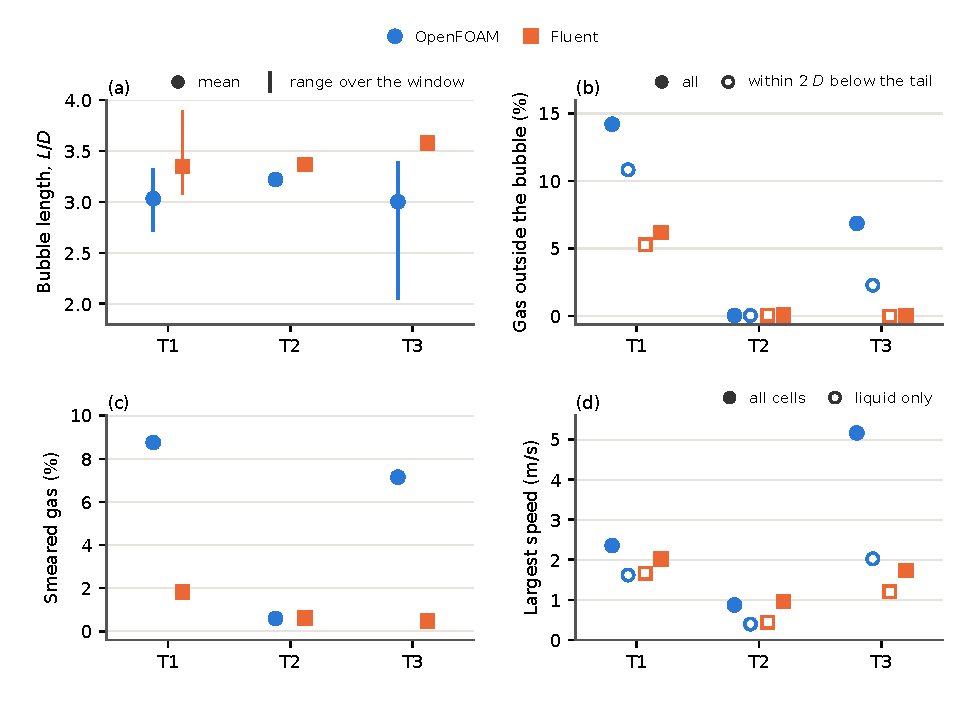
\includegraphics[width=\linewidth]{figures/fig_cases2.eps}
\caption{OpenFOAM and Fluent at T1 to T3 over 5 to 20 s. (a) Bubble length, mean and range. (b) Gas outside the bubble, all (filled) and within 2 $D$ below the tail (open). (c) Smeared gas. (d) Largest speed in all cells (filled) and in the liquid (open).}
\label{fig:cases2}
\end{figure}

\subsection{Validation against the correlations}

Figure~\ref{fig:cases}a and b compare both codes with the reference values. Fr in Fluent lay 0.2\% to 5.3\% from the values of Viana et al.\ and Fr in OpenFOAM 2.7\% to 14.4\%, and all six values lie inside the stated scatter of $\pm 0.05$. At T1 the fine mesh gives Fr = 0.3267, which is 3.5\% below the value of 0.3384. Its film of 0.0655 $D$ over 5 to 20 s is 6.4\% above the value of 0.0615 $D$ from Llewellin et al. On the medium mesh the films at T1 and T2 lie 2.0\% to 6.9\% from that correlation in both codes. At T1 the film in the window was still developing (Section~\ref{sec:film}). Since every result lies inside the scatter, the correlations cannot rank the codes.

\subsection{Rise velocity, film and shape}

Fluent gave Fr 2.5\% above OpenFOAM at T1, 20.8\% above at T2 and 10.7\% below at T3. At T1 this difference is 1.1 times the medium-mesh GCI of about 2.3\%. At T2 and T3 it is 5 to 9 times that value. T3 has no grid study, and at T2 the GCI of the medium mesh was 20.5\% in OpenFOAM and 5.0\% in Fluent. At T2 the bubble kept its gas in both codes and rose at a steady speed. From 5 s to the end of the OpenFOAM run the nose gave Fr = 0.2180 and the centroid 0.2179. At T3 the centroid in OpenFOAM includes the gas lost into the liquid and does not give the bubble speed, so Fr is taken from the nose in both codes. From 5 to 40 s the OpenFOAM nose gave Fr = 0.3150, which is 13.7\% above the value of Viana et al. The fit stops at 40 s, when the nose is 17.5 $D$ above the bottom.

The films agreed within 0.2\% at T1. The Fluent film was 6.1\% thicker at T2 and 6.0\% thinner at T3.

Figure~\ref{fig:shapes} shows the bubble shapes near 20 s, at 20.3, 20.0 and 20.3 s for T1 to T3 in OpenFOAM and 19.7, 20.2 and 20.3 s in Fluent, and Figure~\ref{fig:cases2}a the lengths. The Fluent bubble was longer than the OpenFOAM bubble in all three cases, by 10.5\% at T1, 4.6\% at T2 and 19.3\% at T3. At T1 the length ranged from 2.71 to 3.33 $D$ in OpenFOAM and from 3.08 to 3.89 $D$ in Fluent. At T2 it stayed between 3.20 and 3.24 $D$ in OpenFOAM and between 3.35 and 3.40 $D$ in Fluent. At T3 the Fluent bubble kept a length of 3.54 to 3.64 $D$, while the length of the OpenFOAM bubble rose and fell between 2.04 and 3.39 $D$ over 5 to 20 s. In the long OpenFOAM run it was 3.36 $D$ at 5.3 s and 2.52 $D$ at 39.9 s.

\begin{figure}[H]
\centering
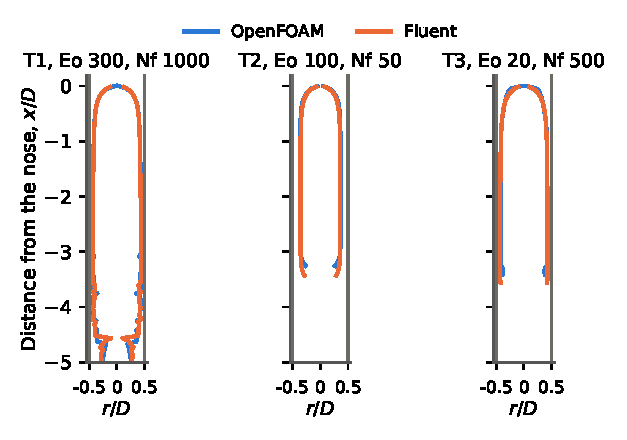
\includegraphics{figures/fig_shapes.eps}
\caption{Interface on the medium mesh near 20 s. Broken lines below the T1 tail are gas shed into the wake.}
\label{fig:shapes}
\end{figure}

\subsection{Gas outside the bubble}

At T1 gas left the tail in both codes, and OpenFOAM held more than twice the share of the gas outside the bubble and in smeared cells that Fluent held (Figure~\ref{fig:cases2}b and c). At T2 neither code lost gas. At T3 the codes differ most, with 6.9\% of the gas outside the bubble in OpenFOAM against 0.006\% in Fluent. In the long OpenFOAM run the smeared share grew from 4\% at 5 s to 18\% at 40 s, spread down to the bottom of the pipe. The larger share of smeared gas and of gas outside the bubble in OpenFOAM comes with its advection scheme. At T1 over 5 to 10 s the momentum predictor alone left the smeared gas and the gas outside the bubble at 4.7\% and 8.8\%, against 4.6\% and 9.3\% in the baseline, while geometric advection with the predictor (Section~\ref{sec:configs}) brought them to 1.4\% and 1.5\%, against 1.4\% and 4.8\% in Fluent. At T3 it cut the smeared gas from 4.3\% to 0.9\%, against 0.5\% in Fluent. This agrees with the sharper interface of geometric reconstruction \cite{horgue2012suitable} and with the lack of convergence of the interface compression of \texttt{interFoam} \cite{cifani2016comparison}.

Figure~\ref{fig:t3fields} shows the two fields at T3 at 20.3 s. At this time the 2 $D$ below the tail held 4\% of the gas in OpenFOAM, half of it detached from the bubble and half in a thin layer along the wall still joined to it, and less than 0.01\% in Fluent. Of the cells in this region faster than 0.3 m/s, 77\% contained gas in OpenFOAM and none in Fluent. Over 5 to 20 s the detached gas in this region averaged 2.3\% of the gas in OpenFOAM and 0.001\% in Fluent. The median of the largest speed over the snapshots was 5.17 m/s in OpenFOAM and 1.73 m/s in Fluent, and 2.03 against 1.20 m/s in the liquid alone (Figure~\ref{fig:cases2}d).

\begin{figure}[H]
\centering
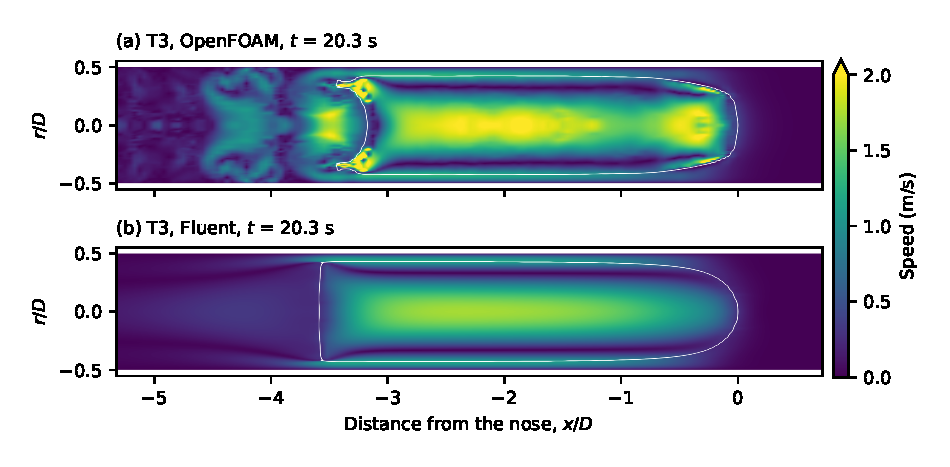
\includegraphics[width=0.75\linewidth]{figures/fig_t3_fields.eps}
\caption{Speed at T3 on the medium mesh at 20.3 s. Speeds above 2 m/s are shown in the top colour.}
\label{fig:t3fields}
\end{figure}

\section{Solver configurations at T2}
\label{sec:configs}

The two codes used the same mesh, fluid properties and time step. They differ in, among others, the interface scheme, MULES in OpenFOAM against Geo-Reconstruct in Fluent, the pressure and velocity coupling, one outer loop in OpenFOAM against 20 iterations per step in Fluent, the pressure interpolation, the density weighting of the surface tension term, and the axisymmetric treatment, a $5^\circ$ wedge against an axisymmetric formulation. At T2, where the codes differ most, these settings were changed one at a time, in one code at a time.

\subsection{Momentum predictor, outer loops and interface advection}

The OpenFOAM runs solve the pressure equation without first solving the momentum equation, with one outer loop per step. At T2 the liquid is 20 times more viscous than at T1, so OpenFOAM T2 was run again to 8.4 s with the momentum equation solved first in each step. Figure~\ref{fig:ladder} gives Fr and the film thickness at T2 for this test and for every other configuration and test at T2. Over 5 to 8.4 s the setting raised Fr by 5.2\% and thickened the film by 1.9\%, and the gap to Fluent fell from 20.5\% to 14.5\%, so the setting accounts for about a quarter of it.

\begin{figure}[H]
\centering
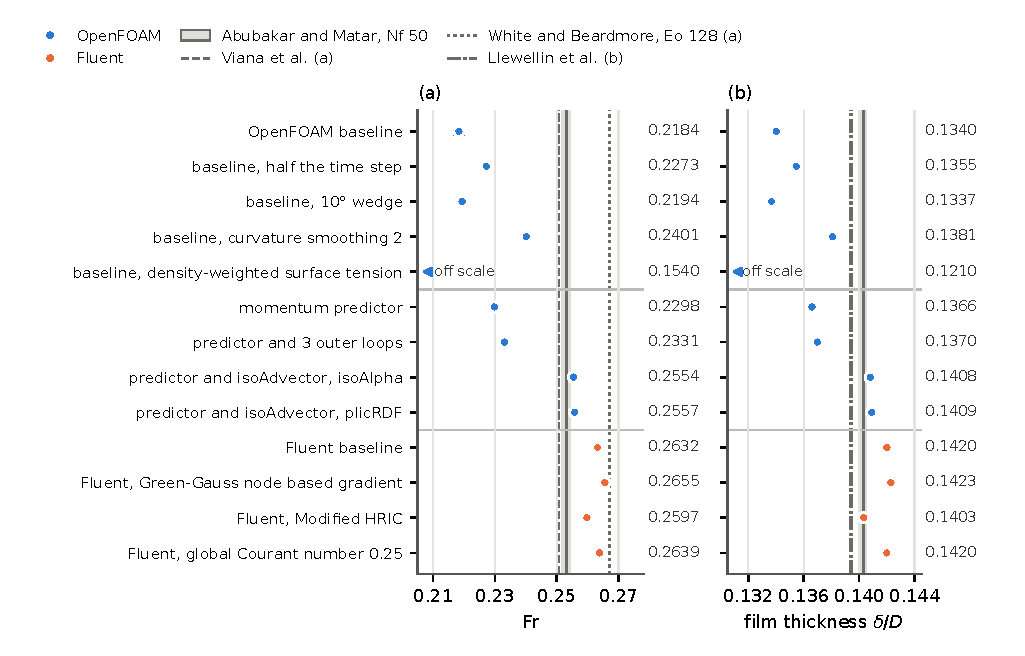
\includegraphics[width=\linewidth]{figures/fig_t2_tests.eps}
\caption{(a) Fr and (b) film thickness at T2 over 5 to 8.4 s for each configuration and test, with the standard error of each fit or mean.}
\label{fig:ladder}
\end{figure}

The published OpenFOAM studies of Gamet et al.\ \cite{gamet2018quantitative,gamet2020validation} solve the momentum equation first, with 1 and 3 outer loops per step. Three more runs at T2 started from the run with the momentum equation solved first and changed one setting each. Two replaced \texttt{interFoam} and its algebraic MULES advection with \texttt{interIsoFoam}, which advects the interface geometrically by the isoAdvector method \cite{roenby2016computational}, once with the isoAlpha reconstruction and once with the plicRDF reconstruction \cite{scheufler2019accurate}. The third kept MULES and took 3 outer loops per step. Each ran to 8.4 s.

Figure~\ref{fig:ladder} gives Fr for each configuration over 5 to 8.4 s. With 3 outer loops Fr rose from 0.2298 to 0.2331, and the gap to Fluent fell from 14.5\% to 12.9\%. With isoAdvector Fr rose to 0.2554 with isoAlpha and to 0.2557 with plicRDF, and the gap to Fluent fell to 3.0\% and 2.9\%. The two reconstructions differ by 0.14\%. Against the steady sharp-interface results of Abubakar and Matar \cite{abubakar2021taylor}, interpolated to Nf = 50, the OpenFOAM baseline lies 13.7\% below, OpenFOAM with geometric advection and the momentum predictor 1.0\% above, and Fluent 4.0\% above. Against the measurement of White and Beardmore the OpenFOAM baseline lies 18.2\% below, OpenFOAM with geometric advection and the momentum predictor 4.3\% below, and Fluent 1.5\% below. Figure~\ref{fig:ladder}b gives the film. The film of the baseline was 4.5\% thinner than the film of Abubakar and Matar and 3.9\% thinner than the correlation of Llewellin et al., the film with the momentum predictor 2.6\% and 2.0\% thinner, the film with geometric advection and the momentum predictor 0.4\% and 1.1\% thicker, and the Fluent film 1.2\% and 1.9\% thicker. At T2 the baseline OpenFOAM result departs from both Fluent and the independent method, while OpenFOAM with geometric advection and the momentum predictor agrees with both within 4\%. This configuration was also run on the coarse mesh, where Fr was 1.5\% higher, and on the fine mesh, where the bubble did not stay in one piece (Section~\ref{sec:grid}).

In the run with 3 outer loops the median initial residual over the 3996 steps from 5 to 8.4 s fell from $5.4\times10^{-3}$ in the first loop to $1.5\times10^{-4}$ in the third for the pressure, and from $1.6\times10^{-3}$ to $5.9\times10^{-5}$ for the radial velocity. The residual of the axial velocity rose from $2.1\times10^{-4}$ to $3.4\times10^{-4}$, and the residual of the volume fraction stayed at $3.6\times10^{-5}$ after the second loop. Three outer loops reduced the pressure and radial velocity residuals by factors of 37 and 27 and changed Fr by 1.4\%, so further outer loops are unlikely to close much of the remaining gap.

\subsection{Surface tension, curvature and the wedge}

Fluent weights the surface tension term by density and OpenFOAM does not (Section~\ref{sec:method}). The OpenFOAM solver was rebuilt with the weight $2\rho/(\rho_l+\rho_g)$ on the surface tension term in the momentum and the pressure equations, with all other settings unchanged. With the weight switched off the rebuilt solver gave the same result as the standard solver over 64 time steps. T2 and T3 were run with the weight from the start to 8.4 s, and the static bubble S to 3.95 s.

At T2 the weight lowered Fr over 5 to 8.4 s by 29.5\%, away from Fluent, and the gap to Fluent grew from 20.5\% to 70.9\%. Fr fell 38.5\% below the value of Viana et al., outside the stated scatter. The film thinned by 9.7\% and the bubble shortened by 8.6\%. The bubble kept its gas, and the gas volume drifted by 0.001\%.

On the static bubble S the weight lowered the mean maximum speed by a factor of about 3, while the liquid peak rose and the pressure jump moved further from the Laplace value of 0.799 Pa. From about 1.6 s the bubble moved along the axis with no gravity, and more of its gas was smeared at the end. So in OpenFOAM the pressure no longer balances the weighted force. The weight is equation (33) of Brackbill et al.\ \cite{brackbill1992continuum}, chosen so that the denser and the lighter fluid in the transition region receive the same acceleration from surface tension. In their static drop tests it increased the error of the pressure jump, slightly with one of their schemes and strongly in poorly resolved calculations with the other, as it did for the static bubble here.

Fluent solves the axisymmetric equations, while OpenFOAM uses a $5^\circ$ wedge one cell thick. A $10^\circ$ wedge with the same cells in the axial and radial directions changed Fr at T2 by 0.5\% (Figure~\ref{fig:ladder}) and started with 2.4\% more gas. OpenFOAM can also smooth the volume fraction before it computes the interface normal (\texttt{nAlphaSmoothCurvature}), and this normal sets both the curvature and the direction of the interface compression. Two smoothing passes on the baseline at T2 raised Fr over 5 to 8.4 s by 10.0\% and thickened the film by 3.0\%, and the gap to Fluent fell from 20.5\% to 9.6\%. A curvature computed from a smoothed volume fraction is not consistent, since its error tends to grow with spatial resolution, and Popinet \cite{popinet2018numerical} considers the method obsolete. Abadie et al.\ \cite{abadie2015combined} report earlier work in which oversmoothing the volume fraction did not allow a bubble rising in liquid at rest to be simulated correctly. So the agreement with Fluent that the smoothing brings is not by itself evidence of a more accurate result.

\subsection{Settings in Fluent}

In Fluent three settings were changed one at a time at T2, each run to 8.4 s (Figure~\ref{fig:ladder}), and each is fitted at the snapshots nearest those of the Fluent baseline. The Green-Gauss node based gradient raised Fr by 0.9\%. The Modified HRIC scheme, which is algebraic, lowered Fr by 1.3\%, and the share of the gas outside the bubble rose from 0.075\% to 0.99\%. A global Courant number of 0.25 changed Fr by 0.3\%. In this last run the time step stayed at its cap, so the Courant limit never acted and the run repeats the medium-mesh run. Against the value of Abubakar and Matar, geometric advection moved OpenFOAM, with the momentum predictor on, from 9.2\% below to 1.0\% above, and the algebraic Modified HRIC scheme moved Fluent from 4.0\% to 2.6\% above. With an algebraic scheme in both codes Fluent still gave a Fr 13.0\% above OpenFOAM, against 2.9\% with a geometric scheme in both. So the type of interface scheme does not by itself explain the gap.

\subsection{The film against laminar film theory}
\label{sec:film}

Below the nose the film can be taken as laminar and developed, with no shear from the gas. Its downward axial velocity is then the profile of Brown that Abubakar and Matar give \cite{abubakar2021taylor},
\begin{equation}
w(r) = \frac{\Delta\rho\, g}{4\mu_l}\left(R^2 - r^2\right) - \frac{\Delta\rho\, g\, a^2}{2\mu_l}\ln\frac{R}{r}, \qquad a = R - \delta,
\label{eq:film}
\end{equation}
where $R$ is the pipe radius and $a$ the radius of the interface. The liquid that the film carries down equals the volume that the bubble sweeps up \cite{llewellin2012thickness}, so the integral of equation~\eqref{eq:film} over the film gives the rise velocity that a film of thickness $\delta$ carries,
\begin{equation}
\mathrm{Fr}_\delta = \frac{\Delta\rho\, g}{8\mu_l a^2\sqrt{gD}}\left[R^4 - 4R^2a^2 + 3a^4 + 4a^4\ln\frac{R}{a}\right].
\label{eq:frfilm}
\end{equation}
The relation of Brown in the form that Llewellin et al.\ and Abubakar and Matar give takes the flux of a flat film over the circumference of the interface, and gives values of Fr 1.2\% to 1.8\% lower at the films of T2.

At T2 the axial velocity of the liquid cells was taken across the film in every column of the film window of the snapshots from 5 to 8.4 s, and compared with equation~\eqref{eq:film} for the film thickness of each column (Figure~\ref{fig:film}a). In the OpenFOAM baseline, with the momentum predictor, with geometric advection and the momentum predictor, and in Fluent, the flux of the cells was 2.2\% to 2.7\% below the flux of equation~\eqref{eq:film}, and the speed of the cell next to the interface 2.7\% to 3.4\% below. Equation~\eqref{eq:film} has no shear from the gas, which the simulations resolve. In every run at T2, in both codes and on all three meshes, Fr lay 0.3\% to 3.3\% below the $\mathrm{Fr}_\delta$ of its own film, and the film was at most 1.0\% thicker than the film that carries the measured Fr (Figure~\ref{fig:film}b). The steady results of Abubakar and Matar at Nf = 40, 60 and 80 lie 1.8\% to 2.0\% below. So at T2 the film in both codes carried the liquid of a developed laminar film of its thickness to within about 3\%, and the configurations of this section moved Fr and the film together along equation~\eqref{eq:frfilm}.

\begin{figure}[H]
\centering
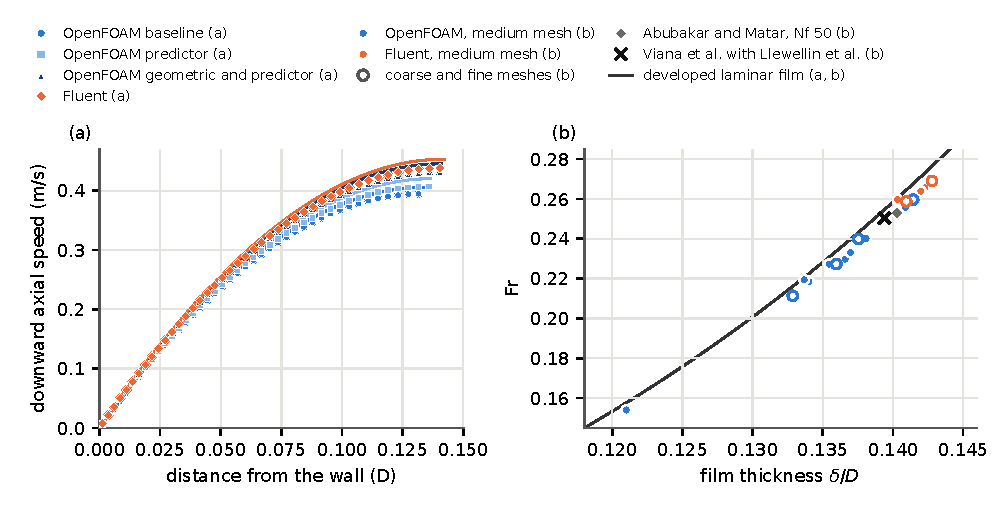
\includegraphics[width=\linewidth]{figures/fig_t2_film.eps}
\caption{The film at T2. (a) Downward axial speed across the film at 8.2 s (8.3 s for the OpenFOAM baseline), 2.1 to 2.2 $D$ behind the nose. (b) Fr against the film thickness over 5 to 8.4 s.}
\label{fig:film}
\end{figure}

At T1 the cells of the film window, 2.0 to 3.4 $D$ behind the nose, carried 76\% to 80\% of the flux of equation~\eqref{eq:film} in the same four configurations, and Fr lay 21\% to 24\% below $\mathrm{Fr}_\delta$ in both codes. So at T1 the film in the window was still developing, and the measured film was 7.7\% to 9.3\% thicker than the developed film that carries the measured Fr. At T3, Fr lay 8\% to 15\% below $\mathrm{Fr}_\delta$. The window starts at the development length $Z$ of Llewellin et al., which takes the film as developed where the speed of the liquid falling from the nose reaches the surface speed of the developed film. With a test on the velocity in the film, Ara\'ujo et al.\ \cite{araujo2012wide} found the film developed about 1.0 $D$ behind the nose below Nf = 90, 2.3 $D$ at Nf = 500 and 2.9 $D$ at Nf = 1000, which at T1 is close to the length of the bubble.

\subsection{Validation uncertainty at T2}
\label{sec:budget}

The comparison at T2 follows the form of the ASME V\&V 20 standard \cite{ASME_VV20}. For a result $S$ and a reference value $D$ the comparison error is $E = S - D$, and the validation uncertainty $u_\mathrm{val} = (u_\mathrm{num}^2 + u_\mathrm{input}^2 + u_D^2)^{1/2}$ combines the numerical uncertainty, the uncertainty from the inputs and the uncertainty of the reference. Table~\ref{tab:budget} gives each part for Fr and for the film, in per cent of the value. The numerical part is the GCI of the medium mesh as it stands. For the OpenFOAM baseline and Fluent it is the GCI of the three meshes (Section~\ref{sec:grid}). For the two configurations with the momentum predictor only the coarse and medium meshes give a value, so it is the two-mesh index of Roache \cite{Roache1994}, $\mathrm{GCI} = 3|\varepsilon|/(r^p - 1)$, with a factor of safety of 3 and an assumed order $p$ of 2 and of 1. The same index is used for the film in Fluent, from the medium and fine meshes. The time step was scaled with the cell size, so the GCI includes the error of the time step. The standard error of the fit of Fr is added to it, and the standard error of the mean film, below 0.2\%, is left out. The inputs are exact in the simulations, and the 0.5\% change of Fr from a $10^\circ$ wedge is added for the wedge of OpenFOAM. For Abubakar and Matar $u_D$ holds the reading of their figures and the interpolation to Nf = 50, 0.6\% for Fr and 0.2\% for the film, and not the 3.4\% by which their Fr missed the measurement of Bugg and Saad. For White and Beardmore it holds the 0.9\% change of the correlation of Viana et al.\ between Eo = 128.4 and 100. No uncertainty is stated for the measurement itself or for the correlation of Llewellin et al.

\begin{table}[H]
\centering
\small
\caption{Validation at T2 on the medium mesh, in per cent of the value. Two values give an assumed order of 2 and of 1.}
\label{tab:budget}
\setlength{\tabcolsep}{4pt}
\begin{tabular}{lcccc}
\toprule
 & OpenFOAM & OpenFOAM & OpenFOAM geometric & Fluent \\
 & baseline & predictor & and predictor & \\
\midrule
Fr & 0.2184 & 0.2298 & 0.2557 & 0.2632 \\
$u_\mathrm{num}$, GCI & 20.5 & 13.8, 33.1 & 4.9, 11.7 & 5.0 \\
$u_\mathrm{num}$, fit & 0.7 & 0.2 & 0.2 & 0.4 \\
$u_\mathrm{input}$, wedge & 0.5 & 0.5 & 0.5 & \\
$E$, Abubakar and Matar & $-13.7$ & $-9.2$ & $+1.0$ & $+4.0$ \\
$u_\mathrm{val}$ & 20.5 & 13.8, 33.1 & 5.0, 11.7 & 5.0 \\
$E$, White and Beardmore & $-18.2$ & $-14.0$ & $-4.3$ & $-1.5$ \\
$u_\mathrm{val}$ & 20.5 & 13.8, 33.1 & 5.0, 11.7 & 5.1 \\
\midrule
Film $\delta/D$ & 0.1340 & 0.1366 & 0.1409 & 0.1420 \\
$u_\mathrm{num}$, GCI & 2.5 & 2.2, 5.3 & 1.2, 2.9 & 2.5, 6.0 \\
$E$, Abubakar and Matar & $-4.5$ & $-2.6$ & $+0.4$ & $+1.2$ \\
$u_\mathrm{val}$ & 2.5 & 2.2, 5.3 & 1.2, 2.9 & 2.5, 6.0 \\
$E$, Llewellin et al. & $-3.9$ & $-2.0$ & $+1.1$ & $+1.9$ \\
\bottomrule
\end{tabular}
\end{table}

For Fr, $|E|$ is smaller than $u_\mathrm{val}$ in every configuration against both references, except for the momentum predictor alone against White and Beardmore with $p = 2$, where they are 14.0\% and 13.8\%. So on the medium mesh the GCI of Fr is as large as the differences, and Fr does not separate the configurations from the references. The direction of refinement does. The Fr of the OpenFOAM baseline fell from 0.2266 to 0.2184 and 0.2116 on the three meshes, away from both references, and extrapolates to 0.1826, 27.9\% below Abubakar and Matar. The Fr of Fluent fell from 0.2696 to 0.2632 and 0.2592 and extrapolates to 0.2527, 0.2\% below them. For the film $u_\mathrm{val}$ is 1.2\% to 6.0\%. The film of the baseline lies 4.5\% below the film of Abubakar and Matar, outside its $u_\mathrm{val}$ of 2.5\%, and its extrapolated film is 6.4\% below. The film with the momentum predictor lies 2.6\% below, against 2.2\% and 5.3\%. The films with geometric advection and the momentum predictor and in Fluent lie inside their $u_\mathrm{val}$ for both orders.

\section{The same settings at T1 and T3}
\label{sec:transfer}

Figure~\ref{fig:transfer} gives Fr at T1 to T3 for the OpenFOAM baseline, the momentum predictor, geometric advection with the momentum predictor and Fluent. The momentum predictor was also tested at T1 on the medium mesh to 10 s and on the square mesh to 15 s. On the medium mesh Fr changed by 0.3\% and the film by 0.4\%, and the gap to Fluent went from 2.7\% to 2.4\%. On the square mesh Fr over 10 to 15 s changed by less than 0.1\%. Over 5 to 10 s, while the square mesh was still settling, it fell by 2.8\%. With the setting on, the square mesh gave a Fr 2.9\% above the medium mesh over 5 to 10 s, against 6.2\% without it. Without the momentum predictor the viscous and convective terms enter each pressure correction through an operator evaluated from the velocity at the start of the step and then from the previous correction, and with it from a velocity that has already solved the implicit momentum equation. Issa \cite{issa1986solution} showed that the implicit predictor step of PISO always damps errors, while the corrector steps are explicit-like. In a one-dimensional linear analysis the corrector steps in their first form damped errors only for a step below a value comparable to the stability limit of an explicitly differenced momentum equation, and Issa treated the diagonal of the operator implicitly to reduce this. The splitting errors fall quickly as the step is refined. For the viscous term the stability limit of an explicit momentum equation is a diffusion number $\nu\Delta t/\Delta r^2$ of order one in the smallest cell. At the wall of the medium mesh this number is about 3 in the liquid and 30 in the gas at T2, against 0.16 and 1.6 at T1 and 0.09 and 0.9 at T3 (Table~\ref{tab:runs}). Without the momentum predictor the three corrector steps act on the viscous term like three Jacobi sweeps of the implicit equation, and for diffusion in one dimension each sweep leaves at most $2d/(1+2d)$ of the error, with $d = \nu\Delta t/\Delta r^2$. At the wall this leaves about 63\% of the error after three sweeps in the liquid at T2 and about 1.4\% at T1. Halving the time step, which halves these numbers, raised Fr by 4.1\% at T2 and by 0.18\% at T1 (Section~\ref{sec:dt}), close to the 5.2\% and 0.3\% of the momentum predictor. Both changes act on the splitting error, and they moved Fr by similar amounts in each case. No run combined the momentum predictor with the smaller step, and the momentum predictor alone was not run at T3.

\begin{figure}[H]
\centering
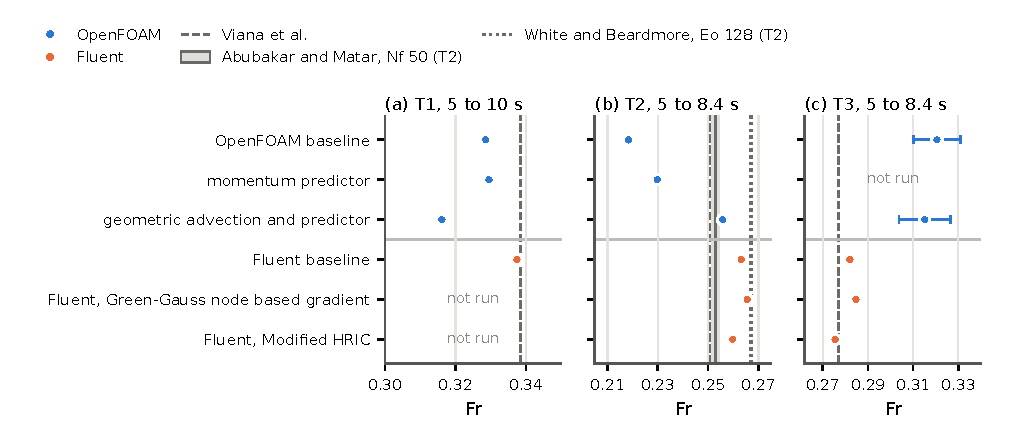
\includegraphics[width=\linewidth]{figures/fig_transfer.eps}
\caption{Fr at (a) T1, (b) T2 and (c) T3 for the same configurations, with the standard error of each fit. The $\pm0.05$ scatter of Viana et al.\ covers every value.}
\label{fig:transfer}
\end{figure}

Geometric advection with the momentum predictor was run at T1 on the medium mesh to 10 s. Over 5 to 10 s it lowered Fr by 3.8\% against the baseline, from 2.9\% to 6.6\% below the value of Viana et al., and the gap to Fluent grew from 2.7\% to 6.7\%. The smeared gas fell by 70\% to about the share in Fluent. The film became 2.7\% thinner, from 6.6\% to 3.8\% above the correlation of Llewellin et al., so the film moved towards that correlation while Fr moved away from the value of Viana et al. At T1 the film in the window was still developing (Section~\ref{sec:film}), and in this run the bubble was 7.2\% longer, so its window reached further behind the nose. The developed film that carries the measured Fr lay 3.6\% below the correlation in this run and 2.4\% below it in the baseline.

At T3 the density weight did not keep a single bubble. The bubble rose more slowly from the start. At 2.2 s its nose was 0.16 $D$ above its starting position, against 0.64 $D$ at 2.26 s without the weight. Up to 2.2 s the gas formed one connected region, and from 2.4 s it split into pieces. At 8.4 s there were 35 pieces, and the largest held 64\% of the gas. The axis held 82 cells with more gas than liquid at the start, 3 at 5 s and none at 6.2 s. At 8.4 s such cells lay from 2.1 to 8.1 $D$ above the bottom, against 4.1 to 7.5 $D$ without the weight at 8.27 s. At 1, 2.4, 5 and 8.4 s the largest speed was 1.43, 7.69, 5.25 and 9.55 m/s, against 4.71 m/s without the weight at 8.27 s, and the largest liquid speed reached 3.77 m/s at 5 s against 1.85 m/s without the weight at 5.26 s. No nose or film could be measured, so no Fr is given. The gas volume drifted by 0.0034\%, and the solver log holds no warnings.

Figure~\ref{fig:transfer}c gives the tests at T3, each fitted at the snapshots nearest those of the baseline in the same code. OpenFOAM with geometric advection and the momentum predictor gave a Fr 1.7\% below the baseline, inside the 3.3\% standard error of the baseline fit, and the smeared gas fell from 4.3\% to 0.9\%. In this run the axis cells inside the bubble alternate between gas and liquid, so its Fr is taken from the highest point of the largest connected gas region, which gives the same Fr as the axis nose for the baseline run at T3. In Fluent the Green-Gauss node based gradient raised Fr by 1.0\% and the Modified HRIC scheme lowered it by 2.3\%, with 1.2\% of the gas outside the bubble against 0.006\% in the baseline. When the window ends earlier these changes lie between 0.4\% and 1.0\% and between 1.7\% and 3.2\%, since the nose speed oscillates and the baseline holds five snapshots in the window. Over the same window Fluent lies 12.0\% below OpenFOAM at T3.


So the OpenFOAM configuration closest to the references at T2 moved Fr away from the value of Viana et al.\ at T1 and left Fr at T3 within the standard error of its baseline. The momentum predictor accounts for about a quarter of the gap to Fluent at T2 and about a tenth at T1.

\section{Limitations}

The grid study covers OpenFOAM at T1 and both codes at T2. T3 was run on the medium mesh without a grid study of its own. The grid studies at T1 and T2 do not carry over to it, since on the same meshes and solver settings the study at T1 converged and the one at T2 did not. The runs are axisymmetric, so the wake and the gas shed at the T1 tail are held symmetric about the axis. The square mesh has about 6 cells across the T1 film against 22 on the medium stretched mesh, so its film value is less resolved. The scatter of $\pm0.05$ stated by Viana et al.\ is 15\% to 20\% of Fr in these cases, and every result in both codes lies inside it, so the correlation alone cannot rank the codes. Mesh shape was tested at T1 only. Curvature smoothing was tested on the OpenFOAM baseline at T2 only. Neither configuration with the momentum predictor gave a Fr on the fine mesh at T2, since the bubble separated, so their grid studies rest on two meshes and their GCI on an assumed order. Geometric advection was run at T1 and T3 on the medium mesh only. The momentum predictor was tested in OpenFOAM at T1 and T2 only, and the density weighting in OpenFOAM at S, T2 and T3 only, to 8.4 s in the rising cases. The spurious currents were measured directly in the static case only, since the peak speed in a rising bubble comes from the flow itself. The bubble length and the gas shares depend on the rule for the tail, the lowest point of the bubble on the axis. The uncertainty of the measurement of White and Beardmore and of the correlation of Llewellin et al.\ is not known, and the uncertainty of the values of Abubakar and Matar covers the reading of their figures only. At T1 the film in the window was still developing, and at T3 Fr lay 8\% to 15\% below the value of a developed film of the measured thickness.
\section{Conclusions}

The grid study at T1 passed for Fr, with a fine-grid GCI of 1.06\% and a GCI of about 2.3\% on the medium mesh. At T2 the grid study of the OpenFOAM baseline gave an observed order of 0.62 and a GCI of 20.5\% on the medium mesh, against an order of 1.44 and 5.0\% in Fluent on the same meshes. A mesh of square cells moved Fr at T1 by 3.6\% in OpenFOAM and by 0.4\% in Fluent, and since it also changes the axial cell and the number of cells across the film, the shift cannot be assigned to the aspect ratio alone. On the static bubble the mean maximum speed was about 5 times higher on the stretched mesh than on a uniform mesh with the same axial cell.

On the same mesh, fluid properties and time step, Fr in Fluent differed from OpenFOAM by +2.5\% at T1, +20.8\% at T2 and $-10.7\%$ at T3. Both codes lie inside the $\pm0.05$ scatter of the correlation of Viana et al.\ in all three cases, so the correlation cannot rank them. OpenFOAM held about twice the share of the gas outside the bubble that Fluent held at T1, and 6.9\% against 0.006\% at T3. This excess comes with its advection scheme, since at T1 the momentum predictor alone left it nearly unchanged while geometric advection brought the smeared gas to the share in Fluent.

At T2, where the codes differed by 20.5\%, the settings were changed one at a time, mostly in OpenFOAM. Solving the momentum equation before the pressure correction in OpenFOAM, which Fluent does in each of its iterations, raised Fr by 5.2\%, about a quarter of the difference, and three outer loops per step changed Fr by a further 1.4\%. With geometric advection in OpenFOAM, Fr came within 4.3\% of the sharp-interface result of Abubakar and Matar, of the measurement of White and Beardmore and of Fluent, and the film within 0.4\% of the sharp-interface film, against 13.7\% and 18.2\% below the two references and a film 4.5\% thinner for the baseline. With an algebraic scheme in Fluent the gap stayed at 13.0\%, so the type of interface scheme does not by itself explain it. Changing the surface tension term of OpenFOAM to the density-weighted form that Fluent uses lowered Fr by 29.5\%, away from Fluent and from both references. Curvature smoothing raised Fr by 10.0\%, but the curvature of that method is not consistent under refinement. The settings tested in Fluent moved Fr by at most 1.3\%.

In every run at T2, in both codes and on all three meshes, Fr lay 0.3\% to 3.3\% below the value that a developed laminar film of the measured thickness carries, so the settings moved Fr and the film together. On the medium mesh the GCI of Fr, 5\% to 33\%, was as large as the differences from the references, so Fr alone does not separate the configurations from them. For the film the uncertainty was smaller. The film of the OpenFOAM baseline lay 4.5\% below the film of Abubakar and Matar, outside its validation uncertainty of 2.5\%, while the films of geometric advection with the momentum predictor and of Fluent lay inside theirs. Under refinement the Fr of the baseline moved away from both references, while the Fr of Fluent moved towards them and extrapolates to 0.2\% below the value of Abubakar and Matar.

The settings that bring OpenFOAM to the references at T2 do not carry over. At T1 geometric advection with the momentum predictor lowered Fr by 3.8\%, from 2.9\% to 6.6\% below the value of Viana et al., and widened the gap to Fluent from 2.7\% to 6.7\%, and at T3 it left Fr within the 3.3\% standard error of the baseline. The momentum predictor moved Fr by 5.2\% at T2 and by 0.3\% at T1, and halving the time step moved it by 4.1\% and 0.18\%. Both act on the splitting error of the PISO algorithm, and the viscous diffusion number of the wall cell was about 3 in the liquid at T2 against 0.16 at T1. The configuration that agrees with the references at T2 is also not confirmed on the grid. On the finest mesh both configurations with the momentum predictor split the bubble, after the pressure residual began to grow at about 0.06 s and a gas flow of up to 122 m/s formed along the axis, while the run without the predictor kept one bubble. Why this happened only on the finest mesh with the predictor was not established.

\clearpage
\paragraph*{Declaration of competing interest}
The author declares no known competing financial interests or personal relationships that could have appeared to influence the work reported in this paper.

\paragraph*{Funding}
This research did not receive any specific grant from funding agencies in the public, commercial, or not-for-profit sectors.

\paragraph*{CRediT authorship contribution statement}
\textbf{Sebbi Adam Kasambula}: Conceptualization, Methodology, Software, Validation, Formal analysis, Investigation, Data curation, Writing -- original draft, Writing -- review \& editing, Visualization.

\paragraph*{Data availability}
The scripts that write and run the OpenFOAM cases, the modified solver, the analysis scripts, the processed results and the source of this paper are available at \url{https://github.com/sebbiakasambula/taylor-bubble-vof}. The OpenFOAM run folders and the Fluent exports are not included because of their size.

\paragraph*{Declaration of generative AI and AI-assisted technologies in the manuscript preparation process}
During the preparation of this work the author used Claude (Anthropic) to help analyse the simulation output and prepare the figures. Claude was also used to revise written text to improve the language. After using this tool, the author reviewed and edited the content as needed and takes full responsibility for the content of the published article.

\paragraph*{Acknowledgements}
I want to give a special thanks to the two women of my life, my mum and my wife. Without their patience and encouragement none of this would be possible. This work used computer resources in the A-house at Link\"oping University.

\bibliographystyle{unsrt}
\bibliography{references}

\end{document}
